\section*{Problem 7}
The goal of this problem is to visualise how similar different animals at a zoo are by projecting the given data from $\mathbb{R}^{16}$ to $\mathbb{R}^{2}$ using three different embeddings; PCA, MDS and Isomap. The data matrix $Y$ will be structured in the same way as in the lecture such that a column of $Y$ corresponds to a data point, thus is $Y \in R^{16 \times 101}$ as there are $101$ data points.

\subsection*{Preprocessing the data}
In order to enable the applications of the embeddings the data has to be preprocessed by first removing the columns 'type' and 'animal name' from the data set. These can later be used in the visualisation.

The remaining attributes are all boolean with values in $\{ 0,1 \}$ except the attribute 'legs' which takes values in $\{ 0, 2, 4, 6, 8 \}$. This attribute thus takes on values up to $8$ times the magnitude in comparison to the remaining attributes which results in the legs attribute to be seen as more important for the embeddings. For this reason the magnitude of 'legs' will be scaled down by $8$ times, causing it to instead take values in  $\{ 0, \frac{1}{4}, \frac{1}{2}, \frac{3}{4}, 1 \}$ giving it a similar magnitude to the remaining attributes.

\subsection*{Visualisation of data}
In order to project the data in 2D such that similar animals are projected close to one another the first two resulting latent variables from a method will be plotted against each other as they contain the most information about the data set as a result of the sorting of the singular values and eigenvalues in descending order.


\subsection*{PCA}
The implementation of PCA was solved in the following manner

\begin{algorithm}[H]
\SetAlgoLined
\KwInput{Data matrix $Y$}
\KwOutput{2-dimensional embedding $X$ }
\KwData{Zoo animals}
 Center the columns (data points) of the data matrix: $Y_c \gets \text{center}(Y)$

 Compute SVD of $Y_c$: $[U,\Sigma, V] \gets \text{SVD}(Y_c)$

 Select the first two columns of $U$: $W \gets [u_1, u_2]$

Compute embedding: $X \gets W^T Y_c$
 \caption{PCA method}
\end{algorithm}


The implementation was quite short using Numpy's Singular Value Decomposition function. The only concern that arised was the centring of the data matrix as it removes the boolean nature of the matrix. However I argue that this only translates the data points and does not remove the information of the attributes which renders the action viable.
\\

The following visualisation was achieved

\begin{figure}[H]
  \centering
  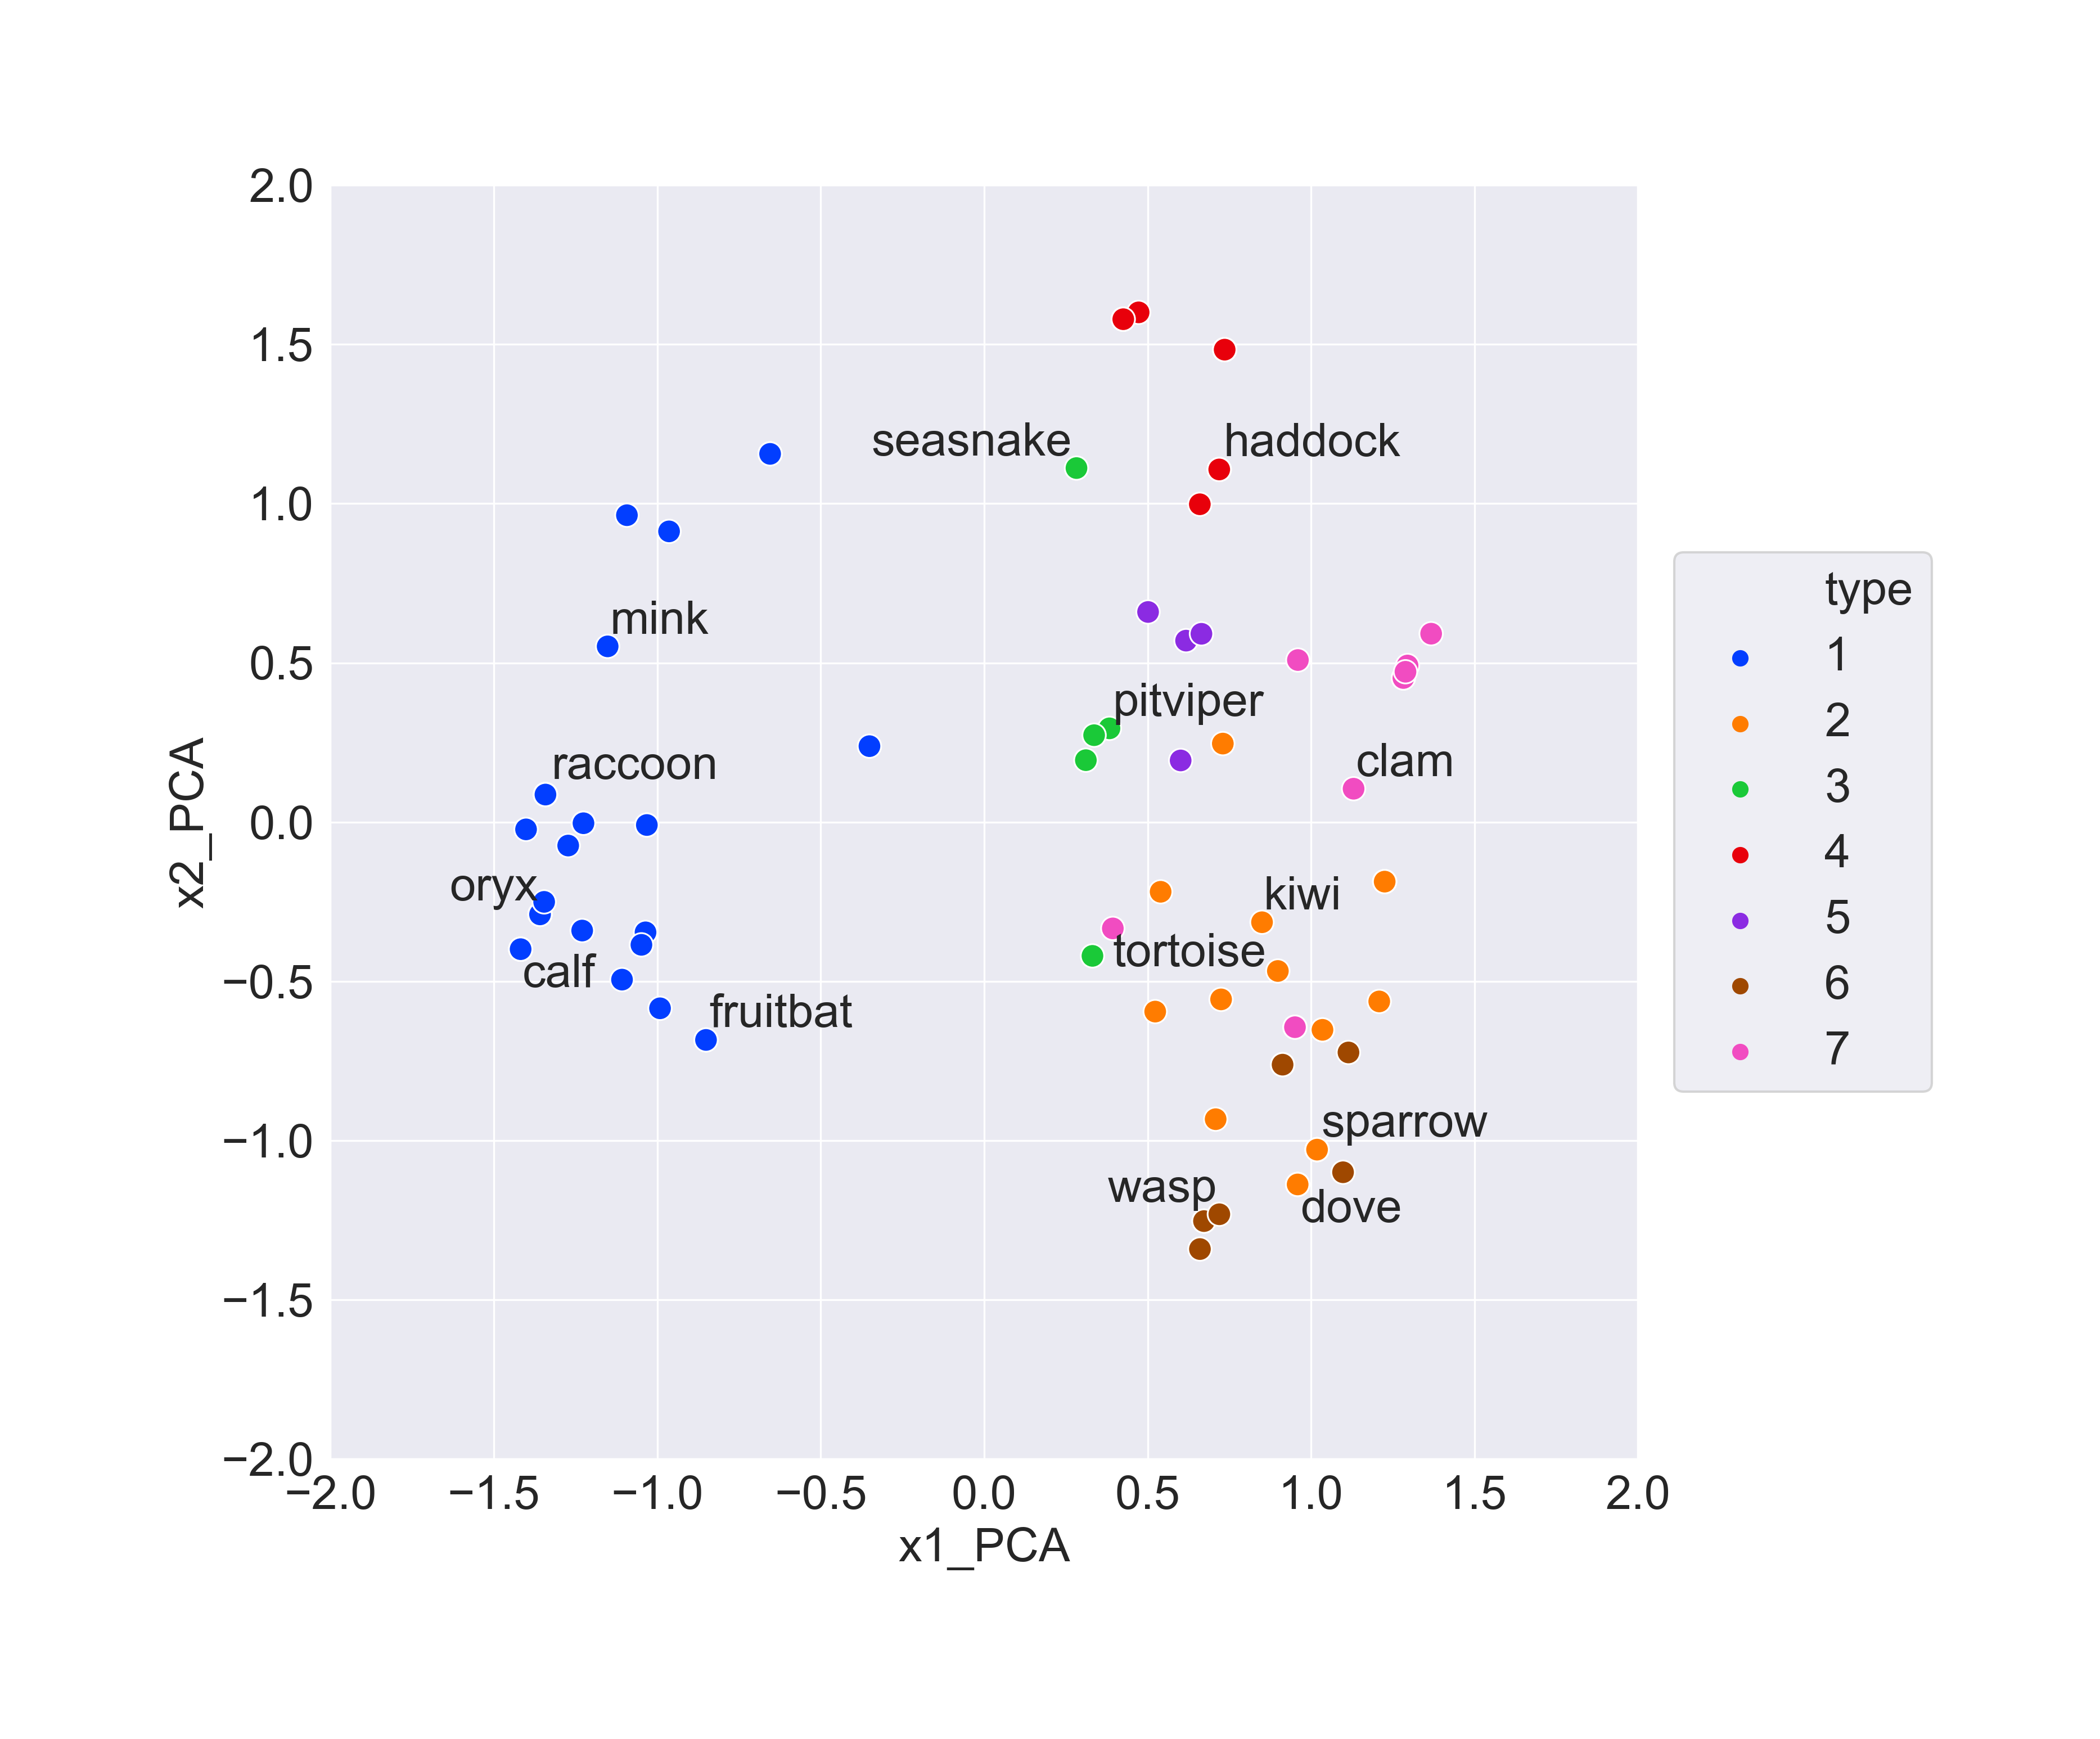
\includegraphics[width = 0.8\linewidth]{../Visualization_PCA.png}
  \caption{Visualisation PCA}
  \label{vis_PCA}
\end{figure}

where a few animals are annotated to give some intuition and understanding behind the placing of the different animals. It is apparent from the plot that there is a clear distinction between type $1$ and the remaining types $2-7$ whom are more mixed among each other.


\subsection*{MDS}
The implementation of MDS was solved in the following manner

\begin{algorithm}[H]
\SetAlgoLined
\KwInput{Data matrix $Y$}
\KwOutput{2-dimensional embedding $X$ }
\KwData{Zoo animals}
  Compute a distance matrix of the data: $D \gets \text{weighted\_distance} (Y) $

  Compute a similarity matrix from $D$: $S \gets \text{similarity\_matrix} (D) $

  Compute Eigen-decomposition of $S$: $[D,Q] \gets \text{Eig}(S)$

  Order $D$ in descending order of eigenvalues magnitude and $Q$ correspondingly

  Ensure elements of $D$ and $Q$ are real

  Compute embedding: $X \gets I_{2\times 101}D Q^T$

  \caption{MDS method}
\end{algorithm}


In the implementation of MDS it was proposed to infer the importance of different attributes by taking it into account when computing the pairwise distance. I solved this by replacing the pairwise distance $d(y_i, y_j)$ with $d_w(y_i, y_j)$ where

\begin{align*}
  & d(y_i, y_j) = \|y_i -y_j \|^2 = (y_i-y_j)^T(y_i-y_j)\\
  & d_w(y_i, y_j) = (y_i-y_j)^T W (y_i-y_j)
\end{align*}

 $y_i, y_j$ are two data points and $W = diag(w_1,w_2,..., w_k)$ where each $w_i$ is a weight for the corresponding attribute. If $w_i = 1, \forall i$ it is the same distance as before but if one weight, lets say $w_1 = 2$ attribute is twice as important as before since if that attribute differs between $y_i, y_j$, that distance is multiplied by $2$ now.

One concern that arose during the implementation of MDS was that the eigenvalues and eigenvectors had small complex components even though the matrix was symmetric. I believe that this was caused by the numerical imprecision of the computer and solved it by simply removing the complex components.

The following visualisations were achieved
\begin{figure}[H]
   \centering
   \begin{subfigure}[b]{0.6\linewidth}
       \centering
       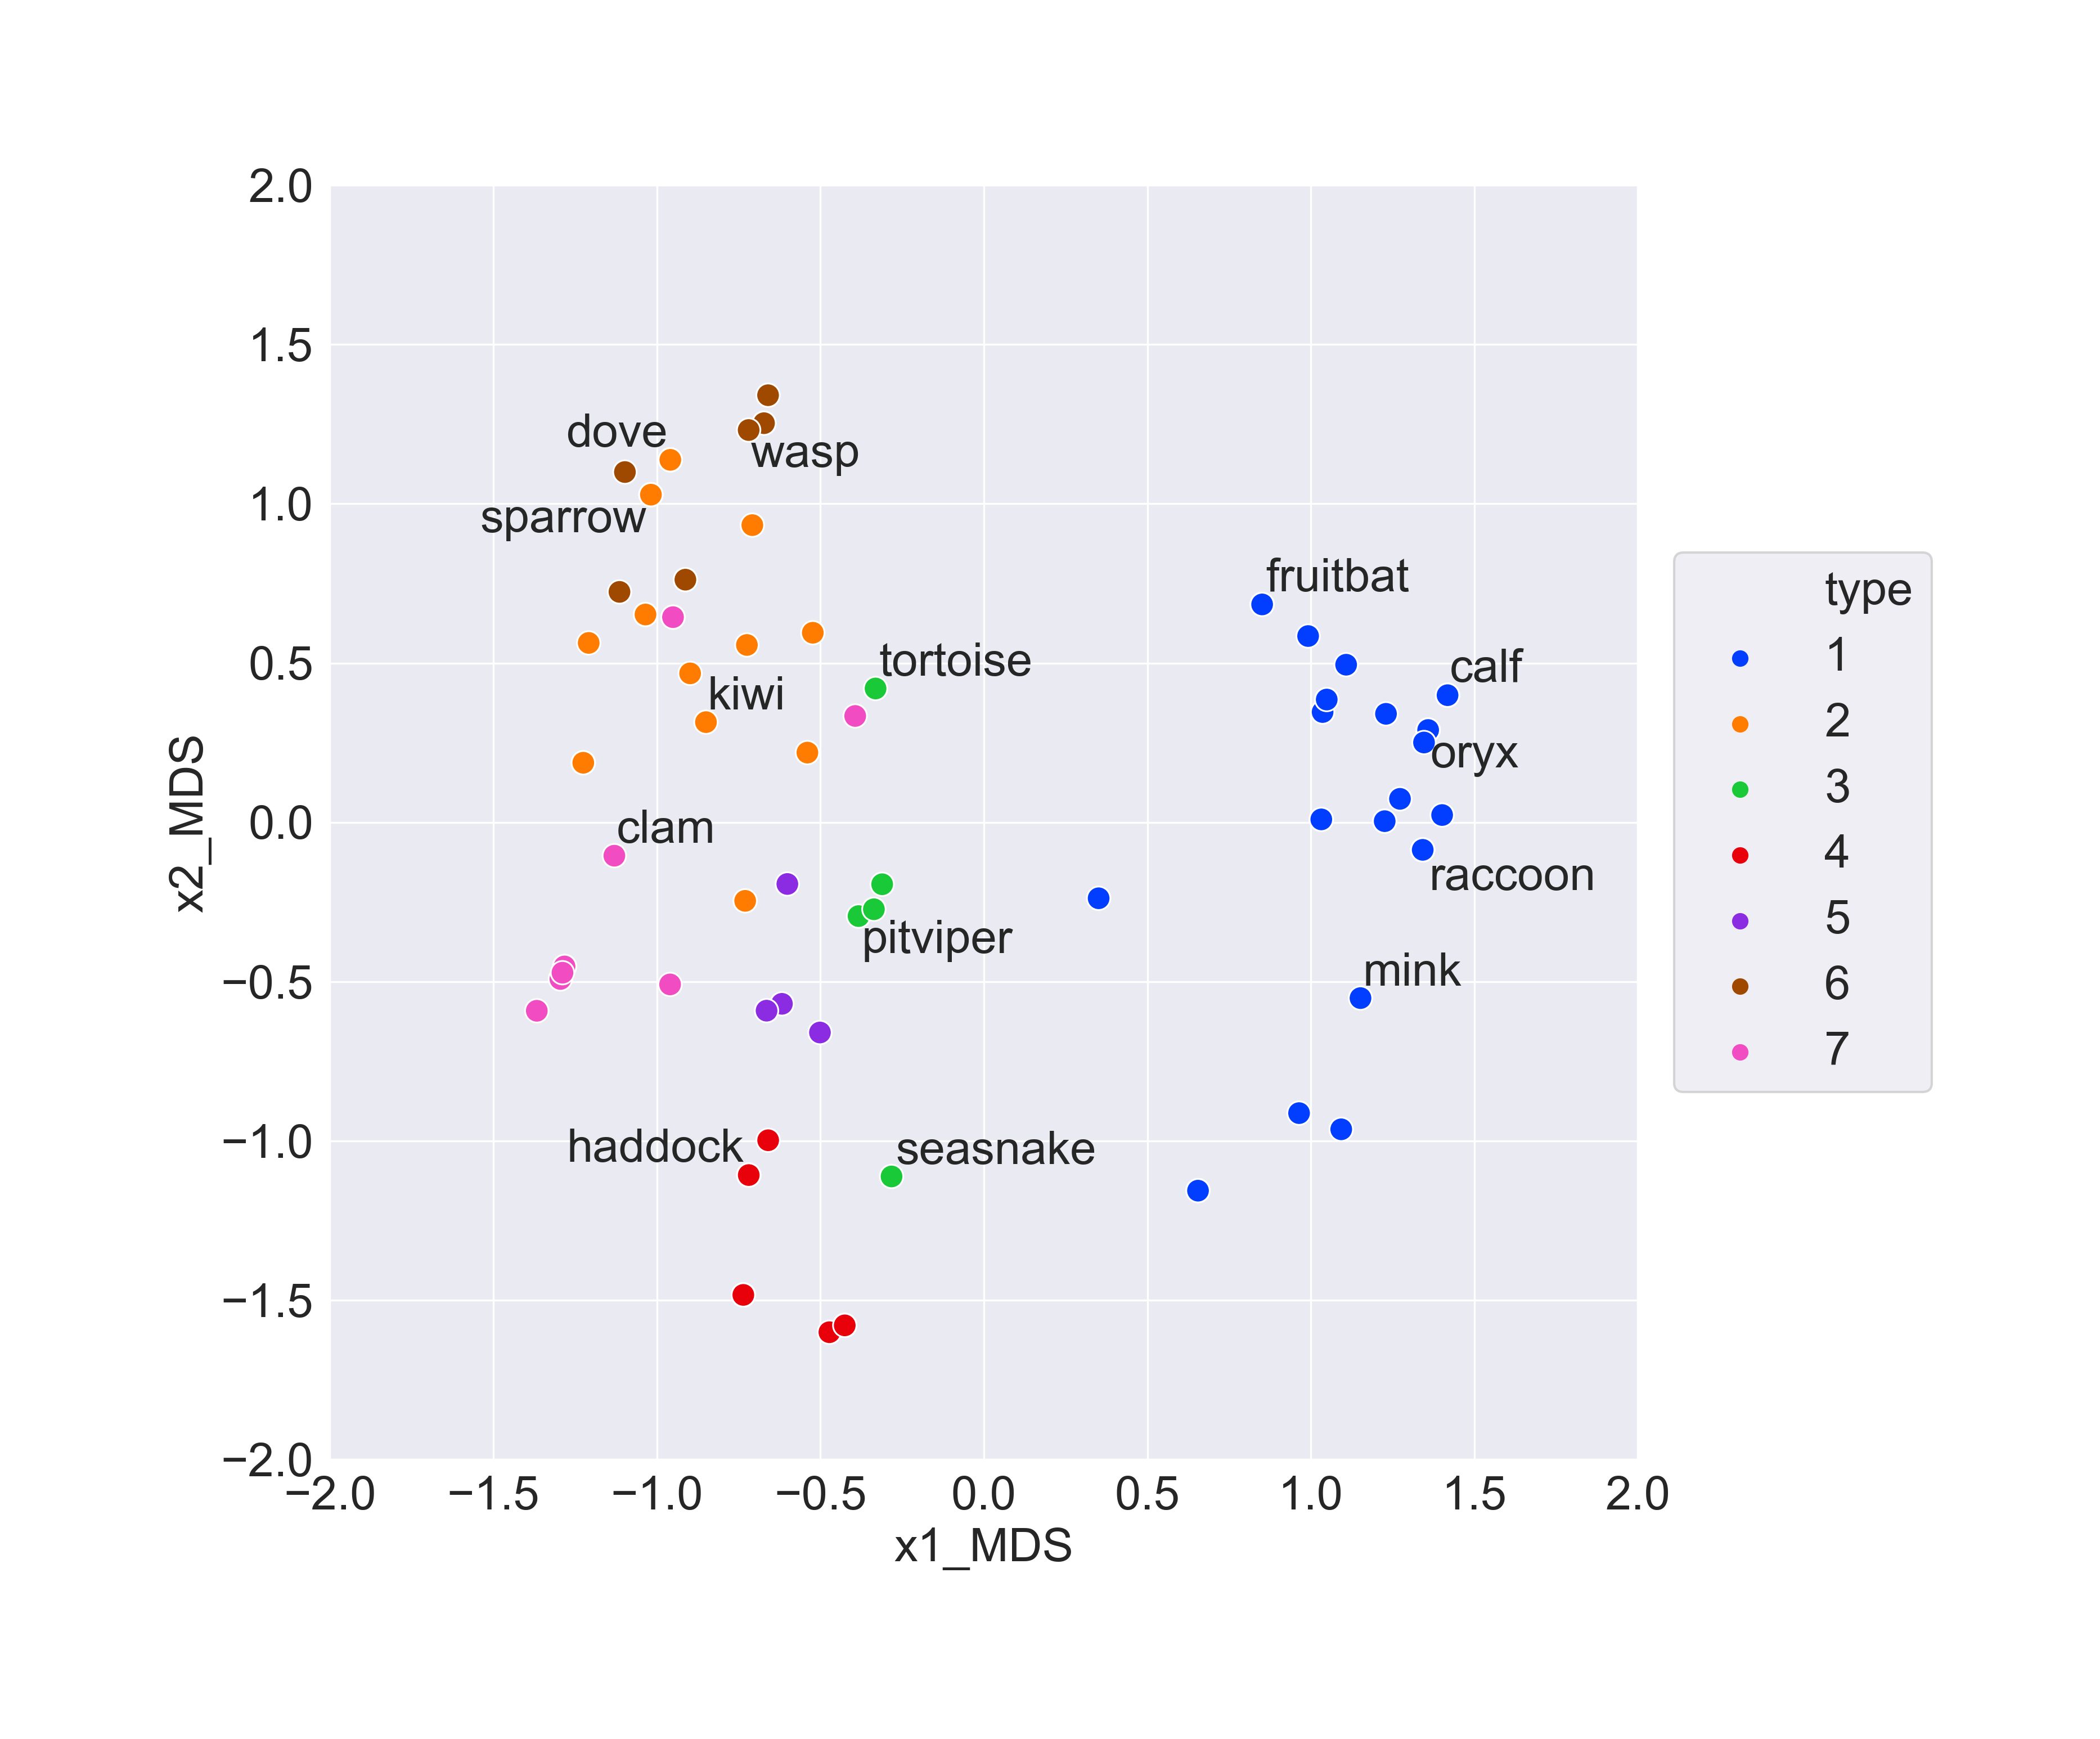
\includegraphics[width=\textwidth]{../Visualization_MDS_no_weights.png}
       \caption{All weights equal to $1$}
       \label{fig:vis_MDS1}
   \end{subfigure}
   \hspace{\fill}
   \begin{subfigure}[b]{0.6\linewidth}
       \centering
       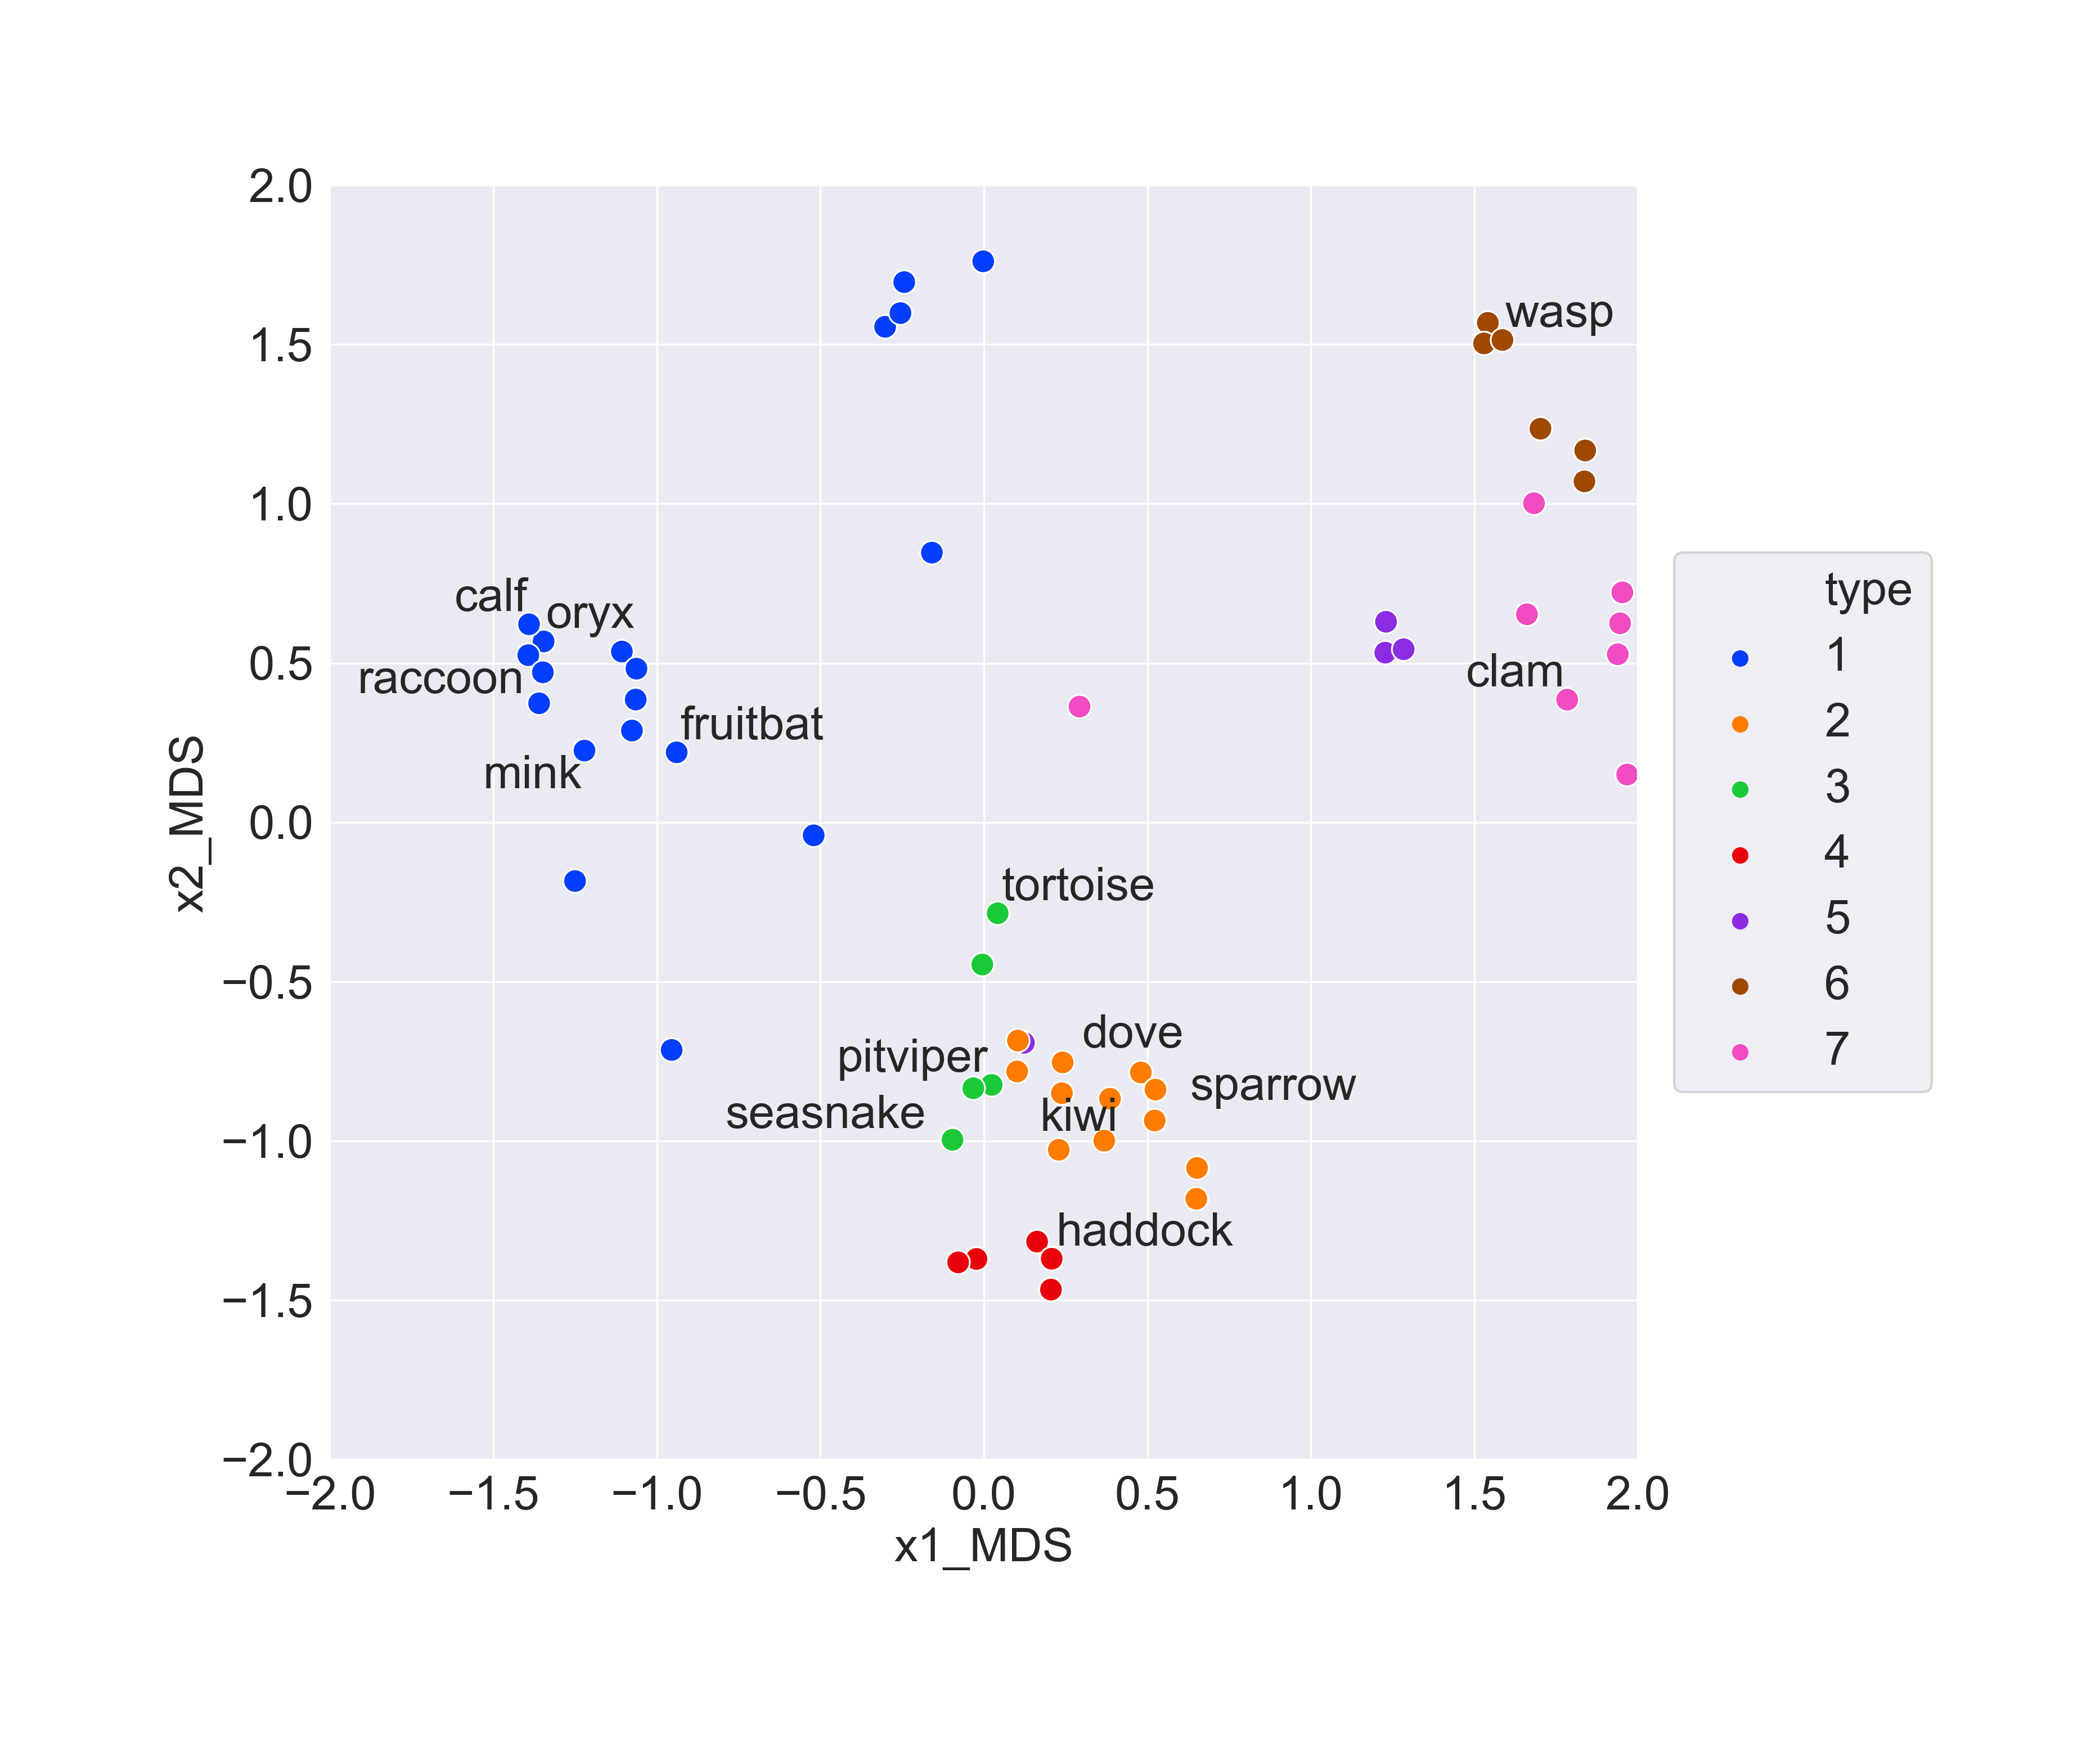
\includegraphics[width=\textwidth]{../Visualization_MDS_with_weights.png}
       \caption{$w_{legs} = 4, \; w_{tail} = 4$, rest equal to $1$}
       \label{fig:vis_MDS2}
   \end{subfigure}
      \caption{MDS method}
      \label{fig:MDS}

\end{figure}
In (\ref{fig:vis_MDS1}) one can see that using all weights equal to $1$ yields a very similar result to the one of PCA only that the points are mirrored over both the y and x axis which I believe is a result of the eigenvalue algorithm of Numpy since one can change the sign of an eigenvector and it still fulfils the eigenvalue equation.

In (\ref{fig:vis_MDS2}) the results become a bit more interesting where I have chosen to put more weight into the number of legs an animal has and whether or not it is has a tail. This has caused further separation of the data and for example the cluster of type $1$ at $(-1.2,0.5)$ seems to have the primal commonality that they all have tails (apparently a fruit bat has a tail) and secondly that they have four legs with the exception of the fruit bat which I believe is why it is in the outer proximity of the cluster.


\subsection*{Isomap}
The implementation of Isomap was solved in the following manner

\begin{algorithm}[H]
\SetAlgoLined
\KwInput{Data matrix $Y$}
\KwOutput{2-dimensional embedding $X$ }
\KwData{Zoo animals}
  Select number of neighbours $k$

  Compute a graph matrix: $G \gets \text{graph\_matrix}(\text{data matrix}, k)$

  Compute shortest path matrix: $P \gets \text{shortest\_path(G)}$

  Compute similarity matrix: $S \gets \text{similarity\_matrix} (P)$

  Compute embedding: $X \gets \text{MDS}(S)$
 \caption{Isomap method}
\end{algorithm}

In order to find the shortest path I used SciPy's implementation of the graph shortest path where I noticed even though all possible neighbours were used the returning distance matrix had a small perturbation in relation to the original distance matrix. A result that is unintuitive to me, however as the perturbations were small the end result was not affected.

The following visualisations were achieved
\begin{figure}[H]
   \centering
   \begin{subfigure}[b]{0.6\linewidth}
       \centering
       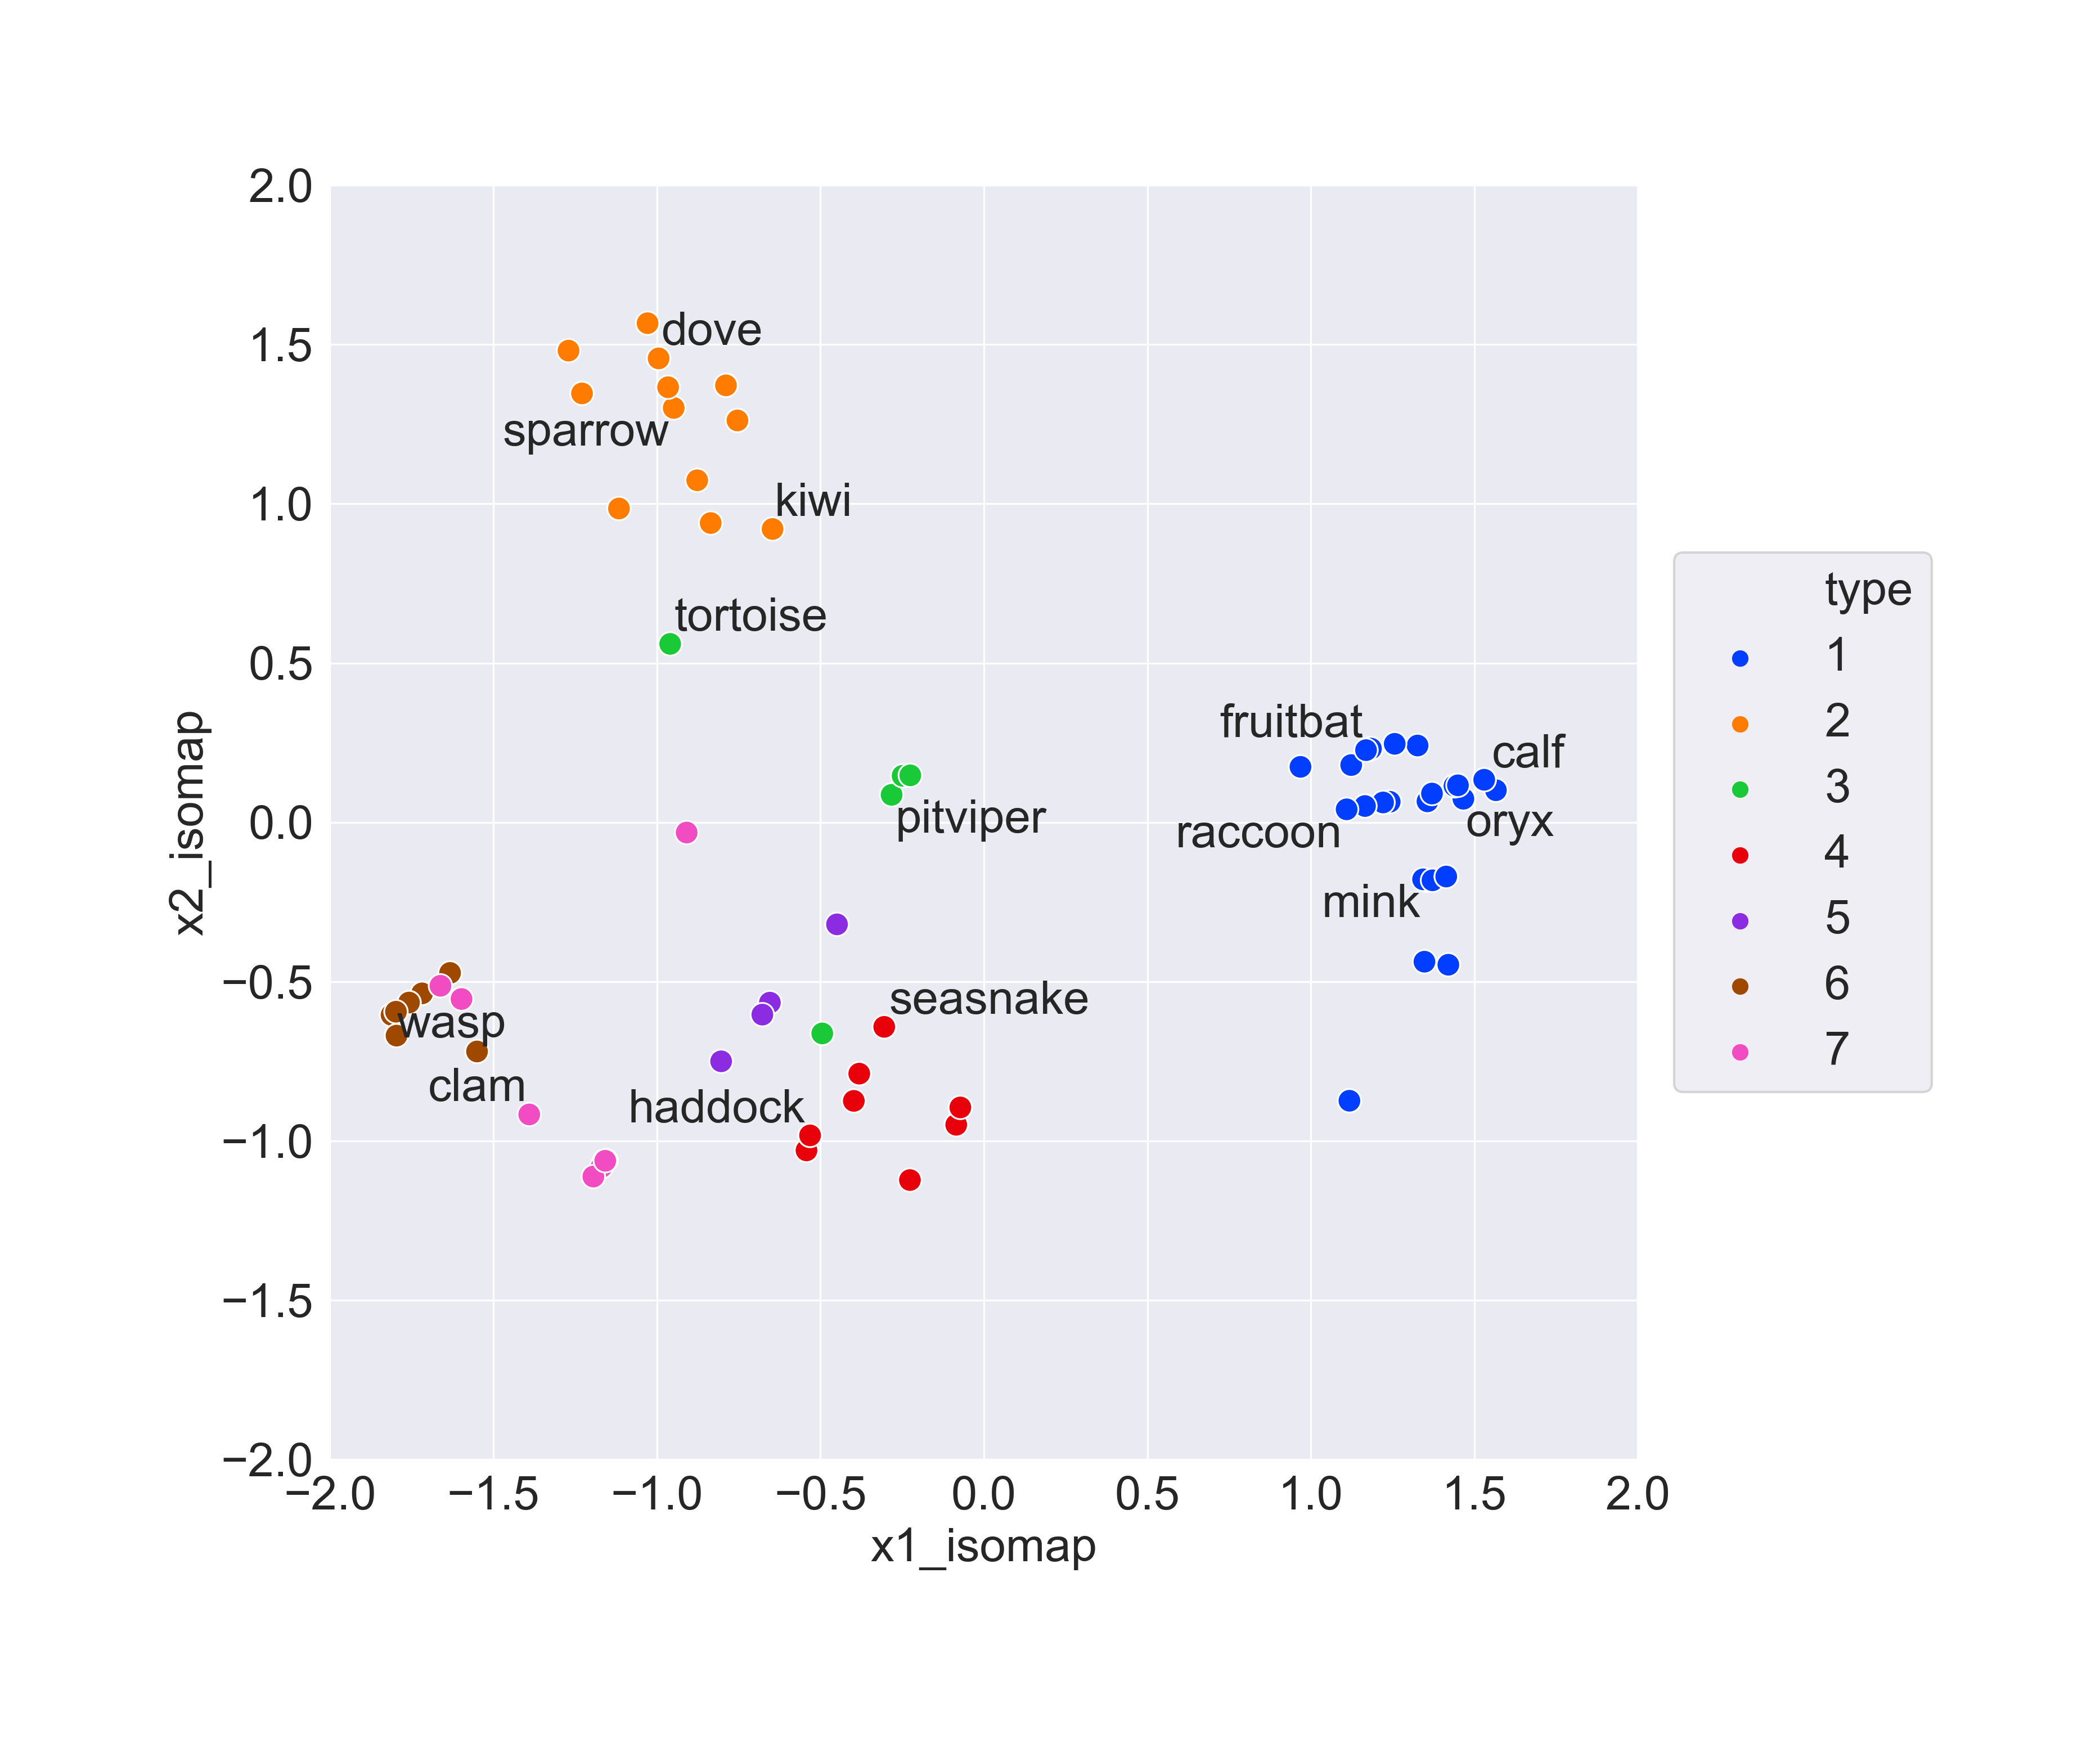
\includegraphics[width=\textwidth]{../Visualization_Isomap_n_10.png}
       \caption{Number of neighbours set to $10$}
       \label{fig:isomap 10}
   \end{subfigure}
   \hspace{\fill}
   \begin{subfigure}[b]{0.6\linewidth}
       \centering
       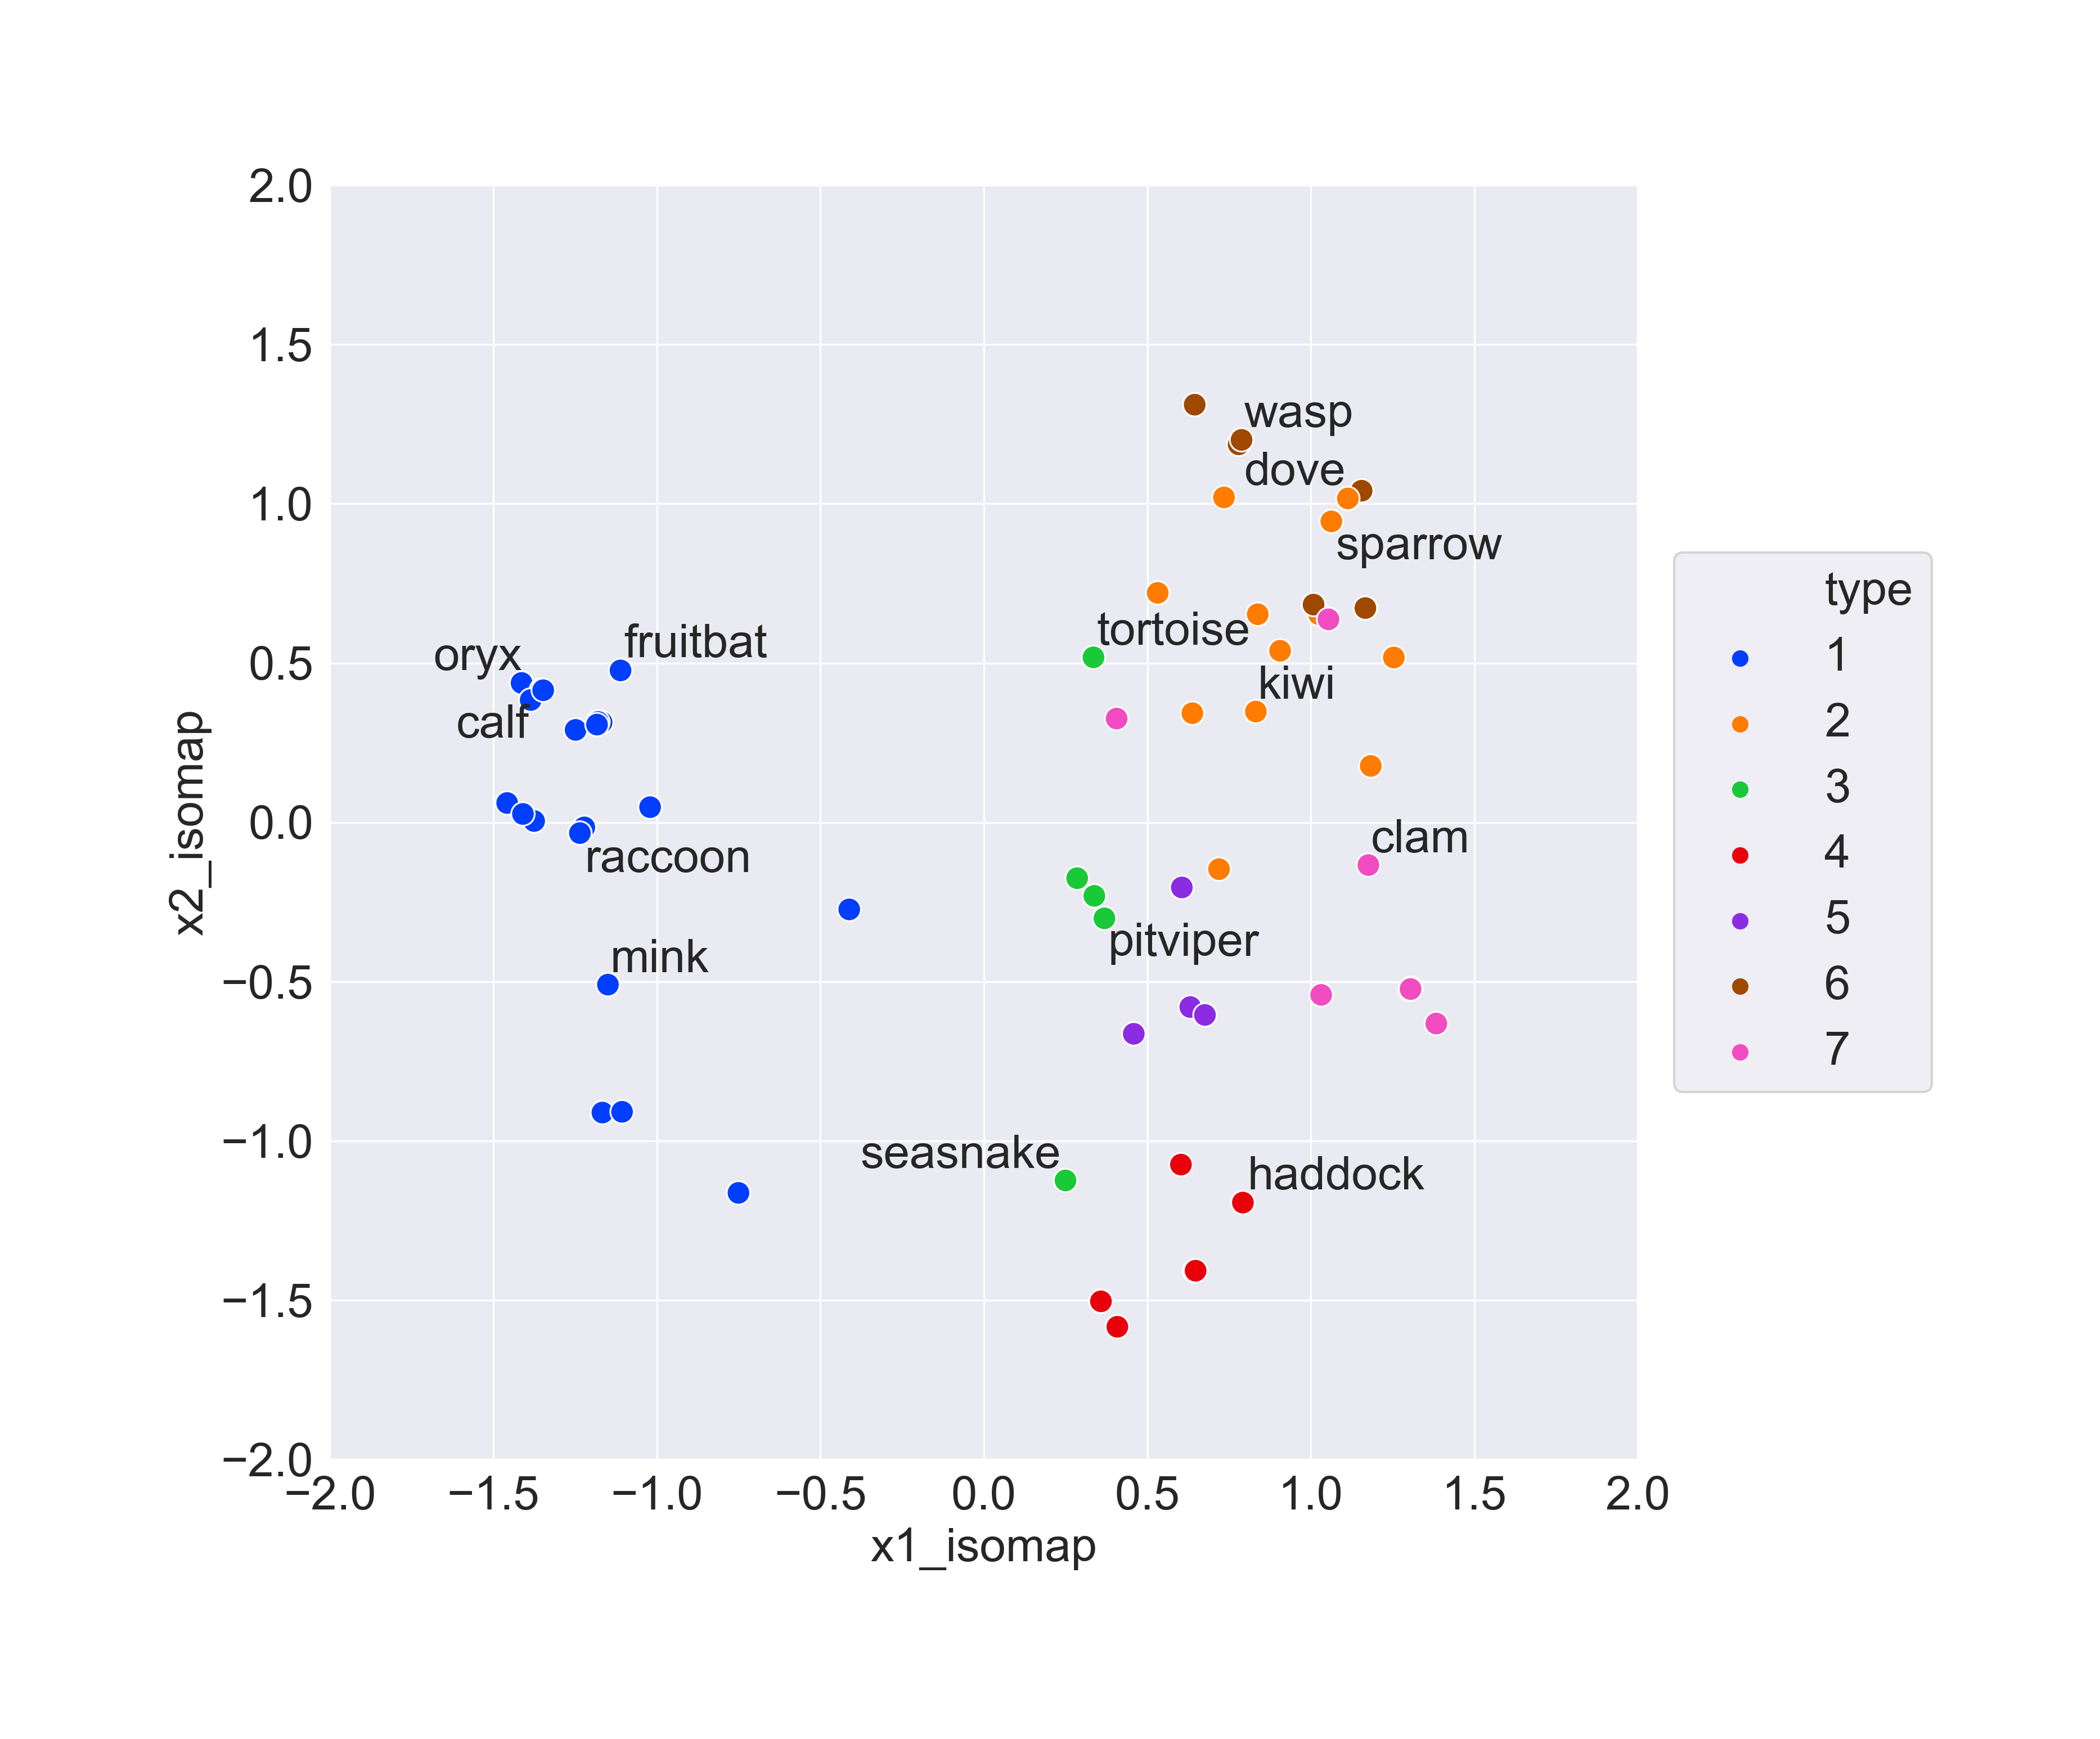
\includegraphics[width=\textwidth]{../Visualization_Isomap_n_30.png}
       \caption{Number of neighbours set to $30$}
       \label{fig:isomap 30}
   \end{subfigure}
      \caption{Isomap method}
      \label{fig:isomap}

\end{figure}

As I mentioned previously Isomap converges to the same result as both MDS and PCA (although with small perturbations) when the number of neighbours are increased. This behaviour can be seen in figure (\ref{fig:isomap 30}) where it has started to converge towards figure (\ref{fig:vis_MDS1}) where MDS has uniform weights. For this reason I opted for a low amount of neighbours in order to capture the structure of the data manifold and the final choice was set to $10$ neighbours which can be seen in figure (\ref{fig:isomap 10}). In figure (\ref{fig:isomap 10}) there is great separation between the different types of animals which gives reason to believe that Isomap captures the underlying structure of the data really well.


\subsection*{Comparison}
The final choice for each method is plotted in the three figures below.

\begin{figure}[H]
  \centering
  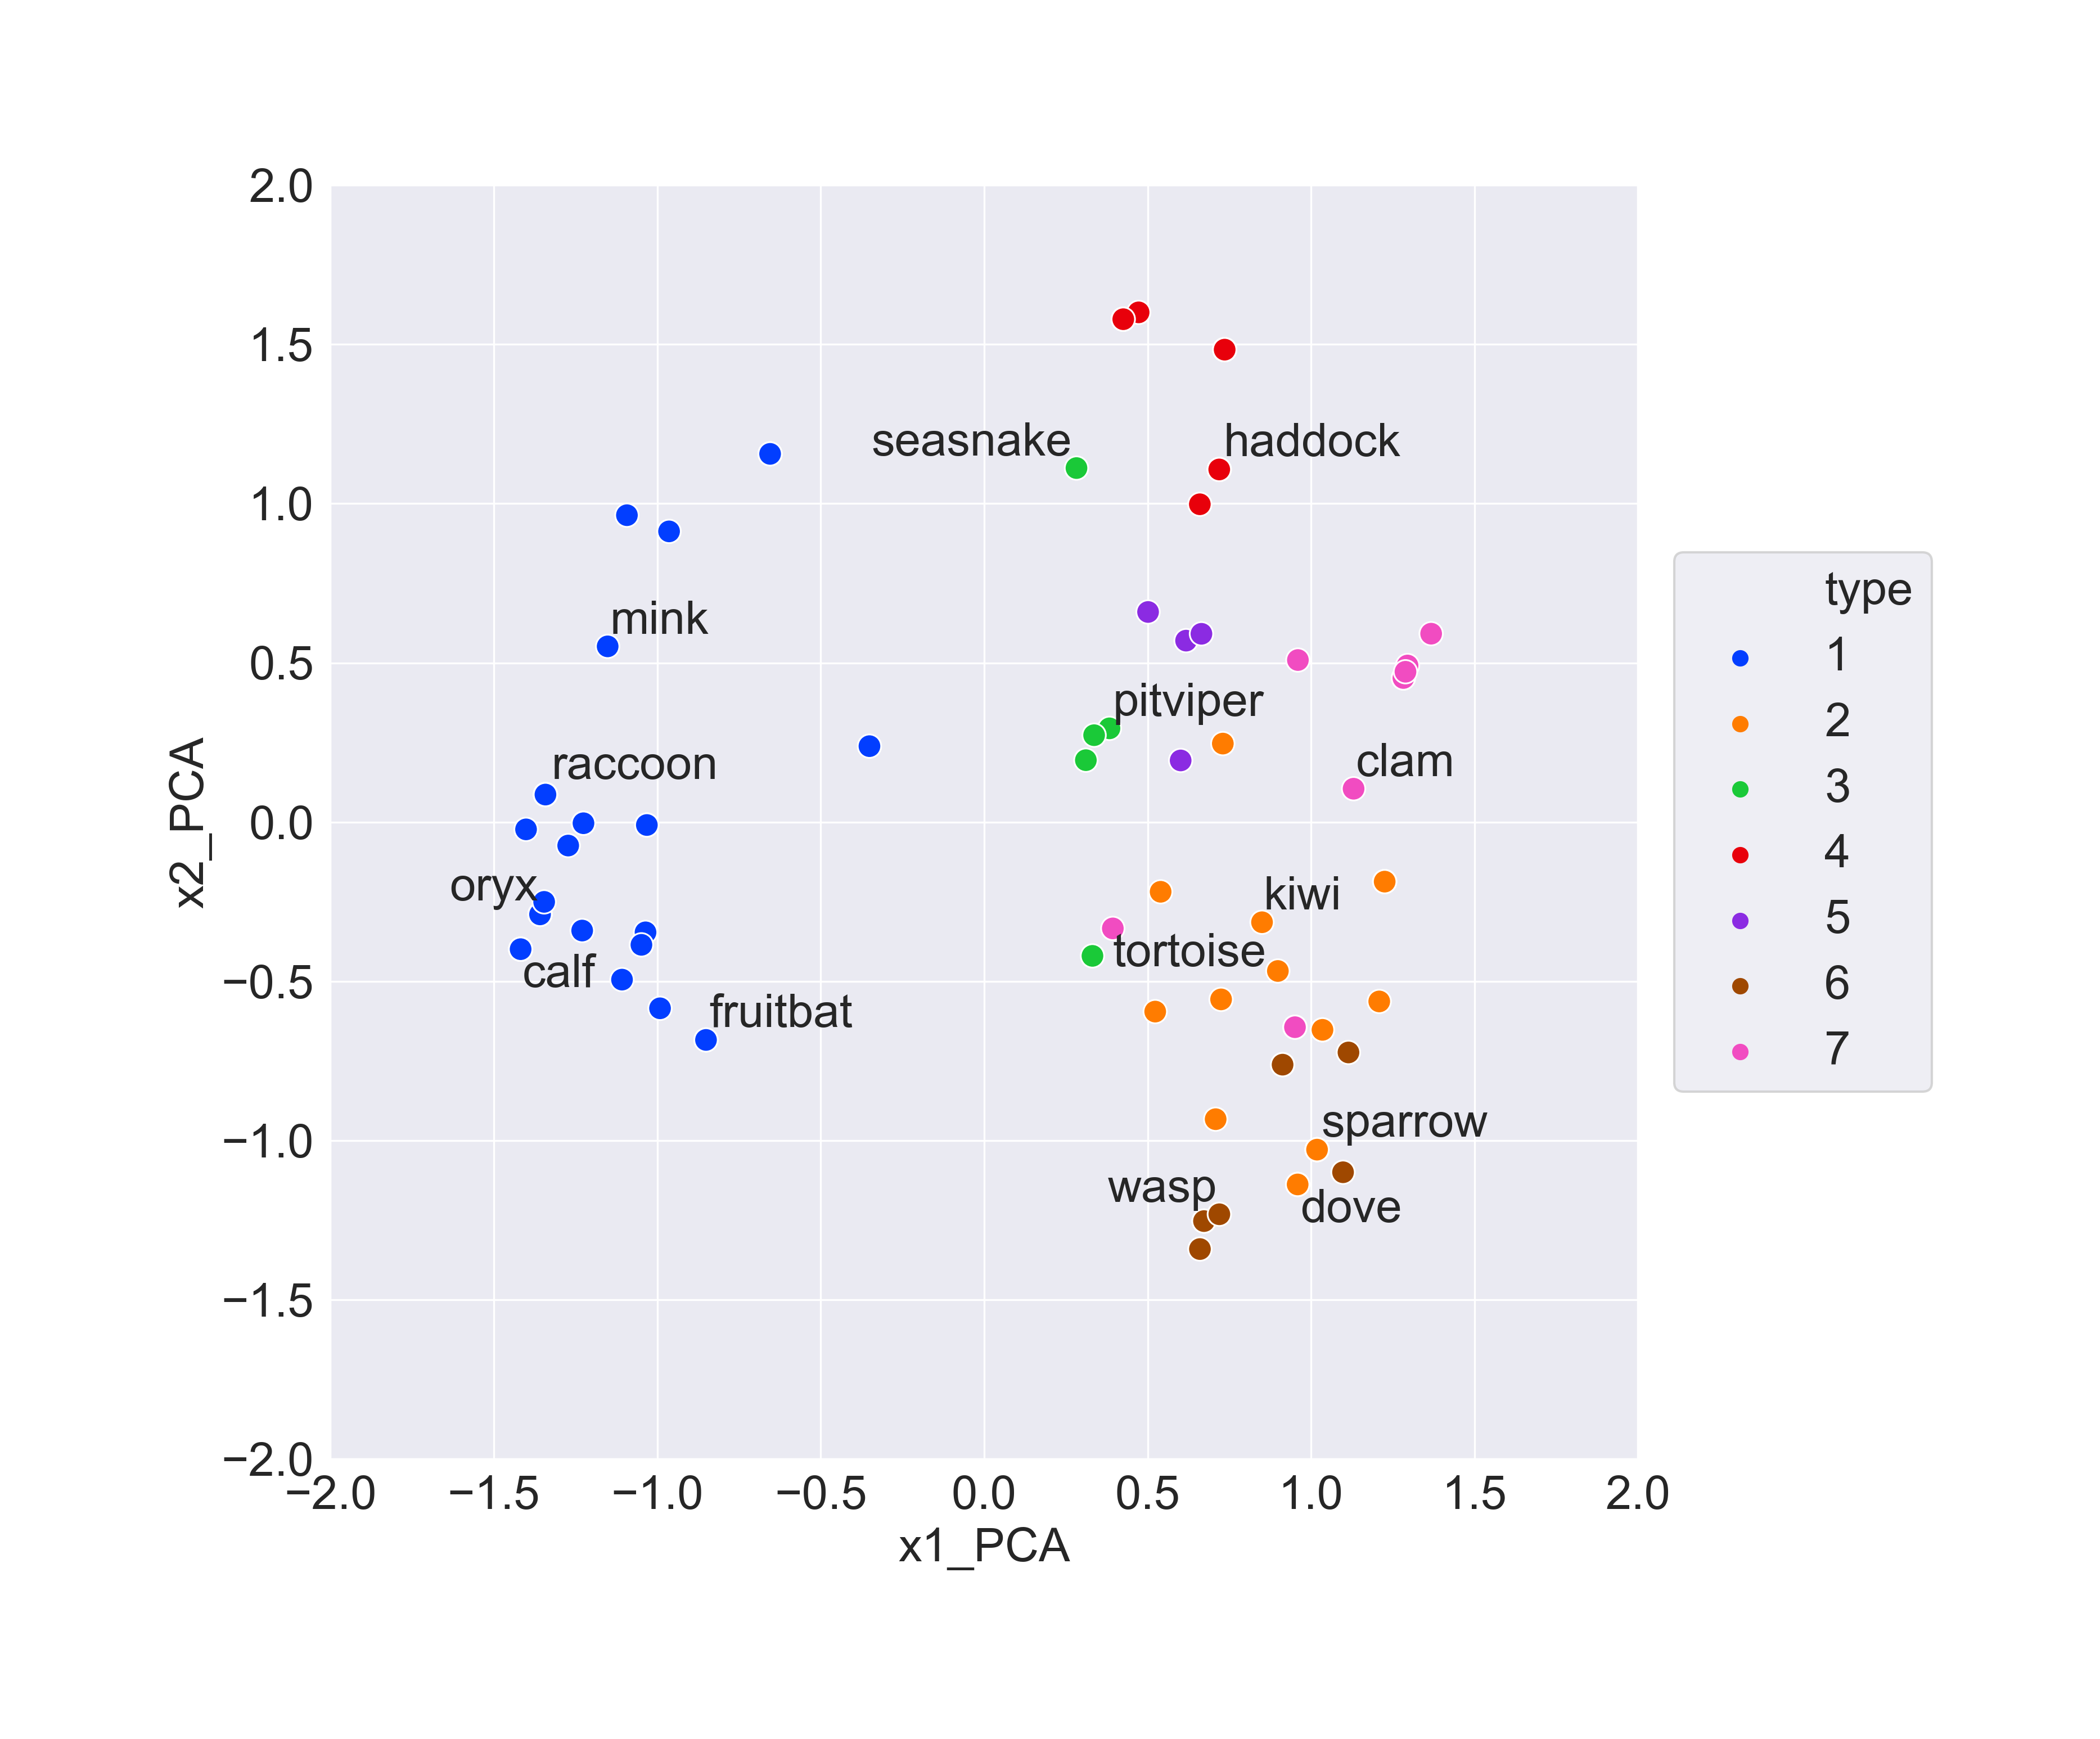
\includegraphics[width = 0.8\linewidth]{../Visualization_PCA.png}
  \caption{PCA}
  \label{fig:PCA final}
\end{figure}

\begin{figure}[H]
  \centering
  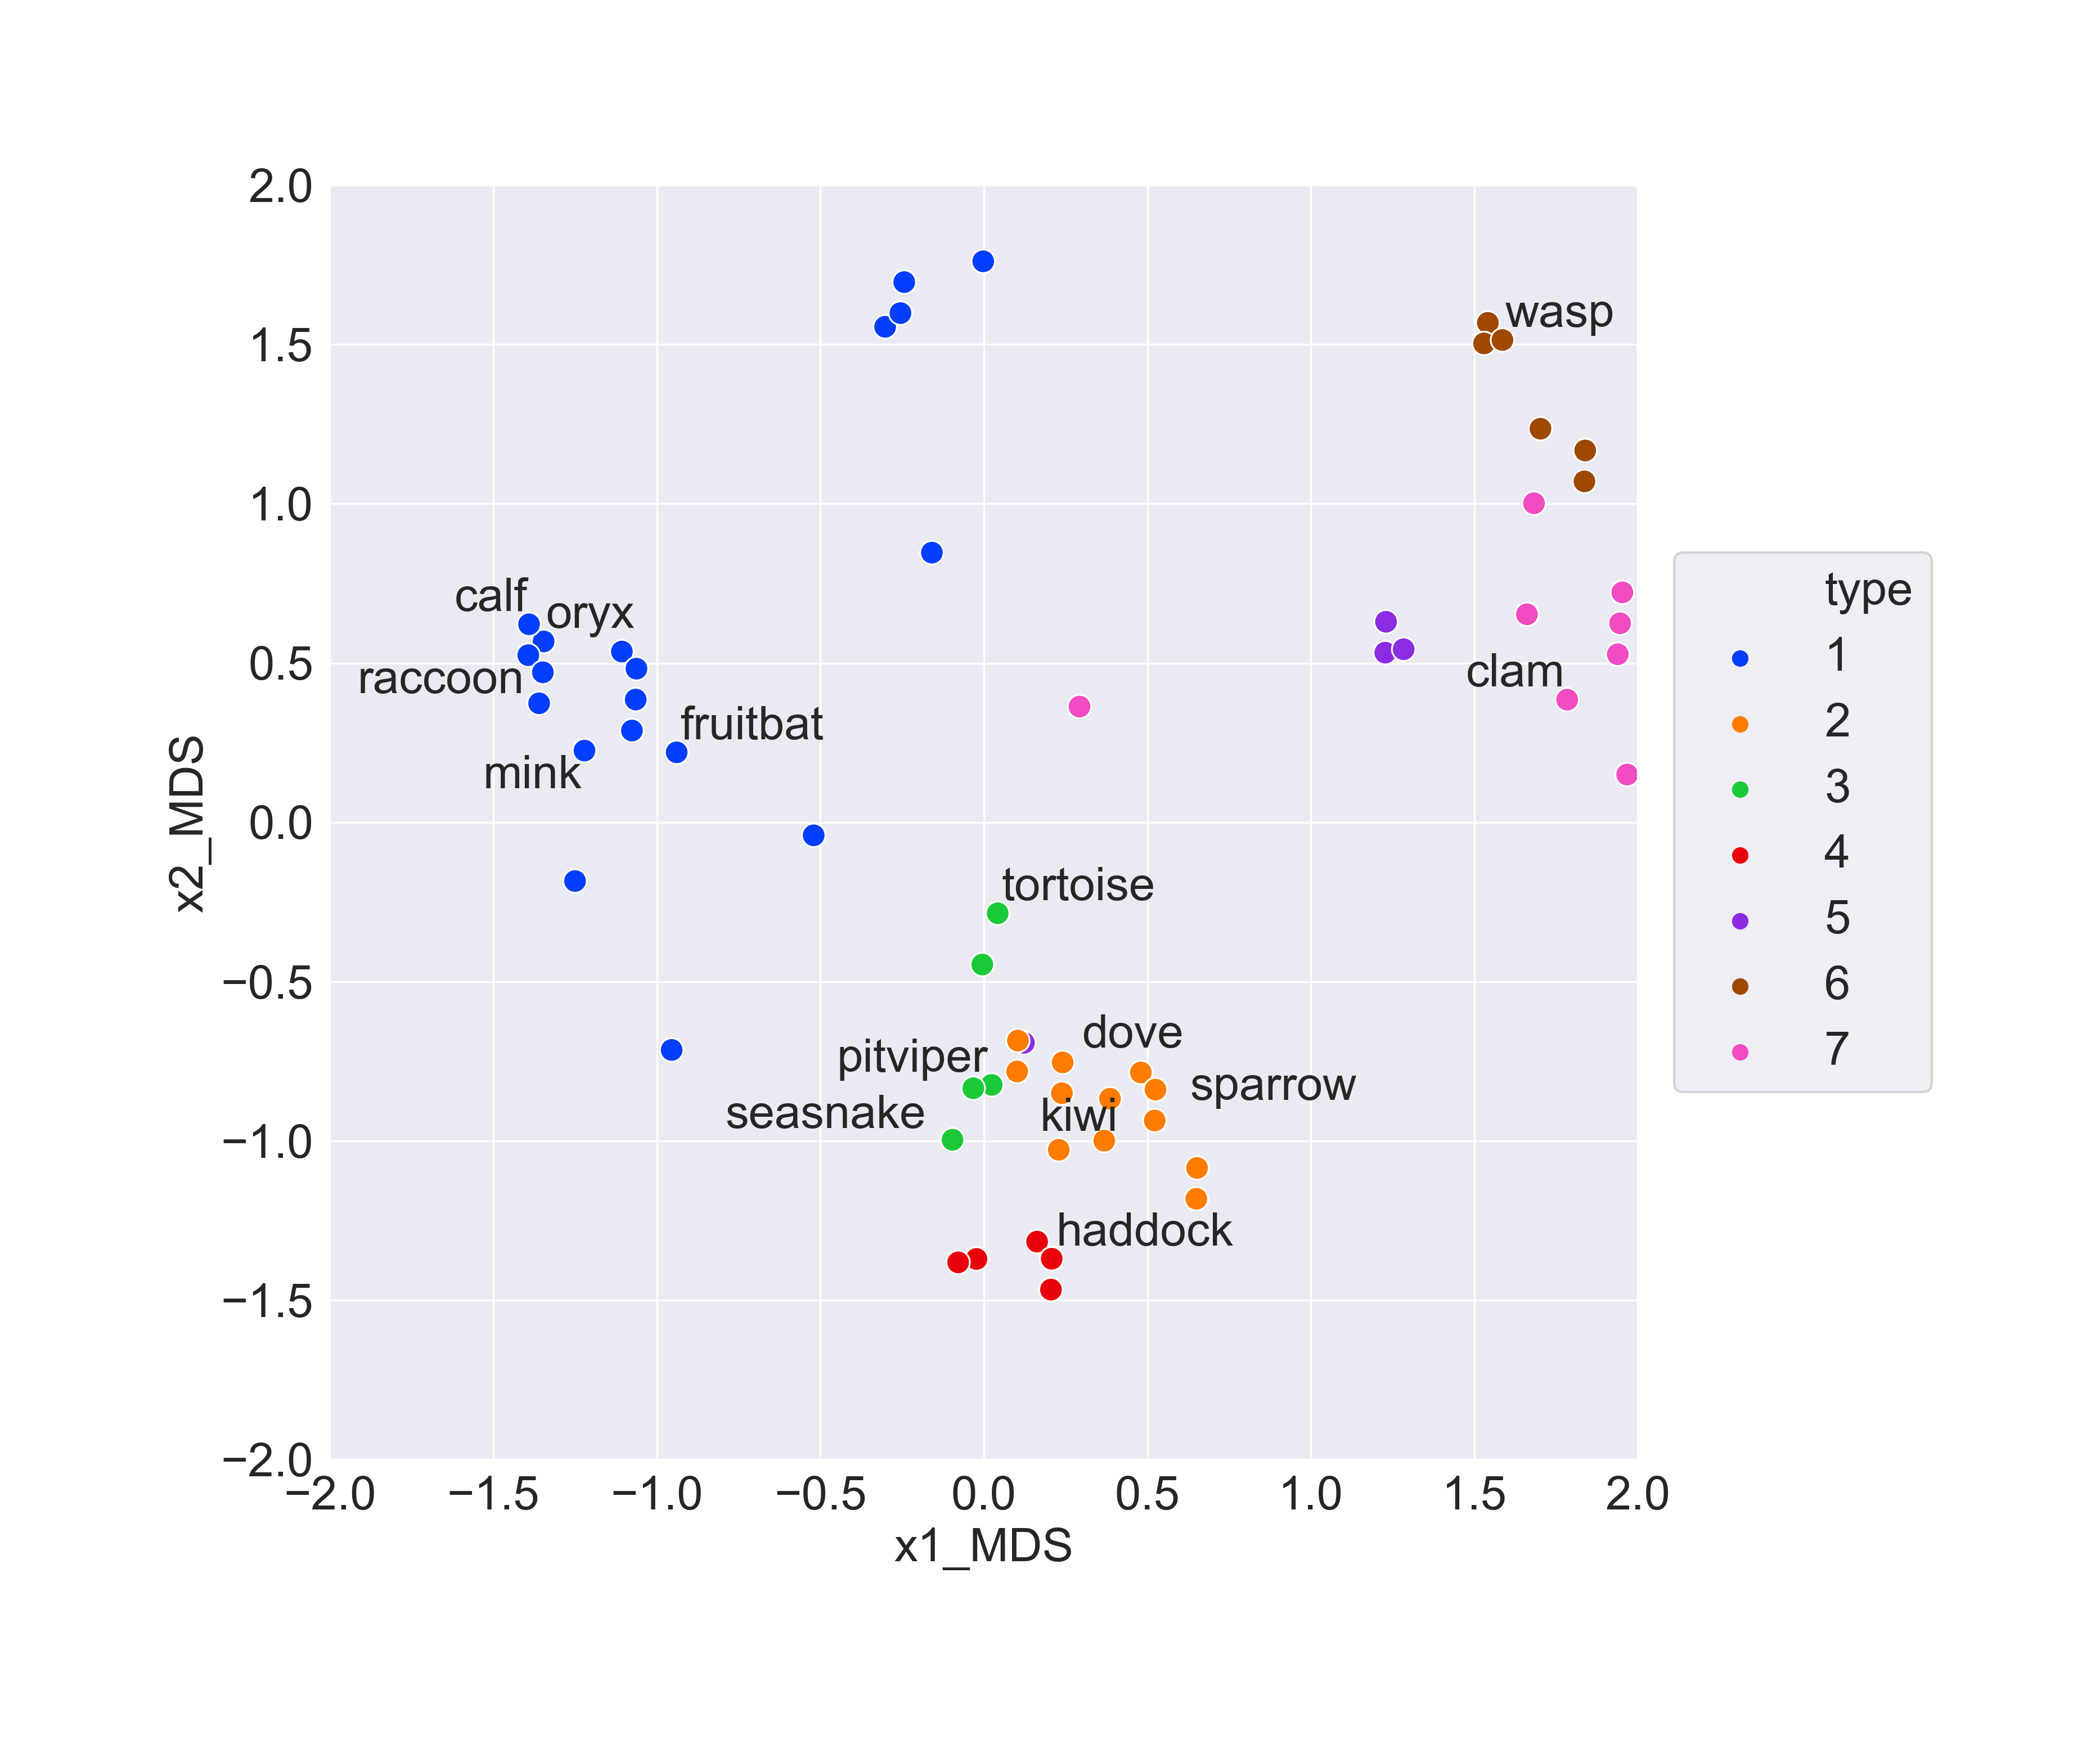
\includegraphics[width = 0.8\linewidth]{../Visualization_MDS_with_weights.png}
  \caption{MDS, $w_{legs} = 4, \; w_{tail} = 4$, rest equal to $1$}
  \label{fig:MDS final}
\end{figure}

\begin{figure}[H]
  \centering
  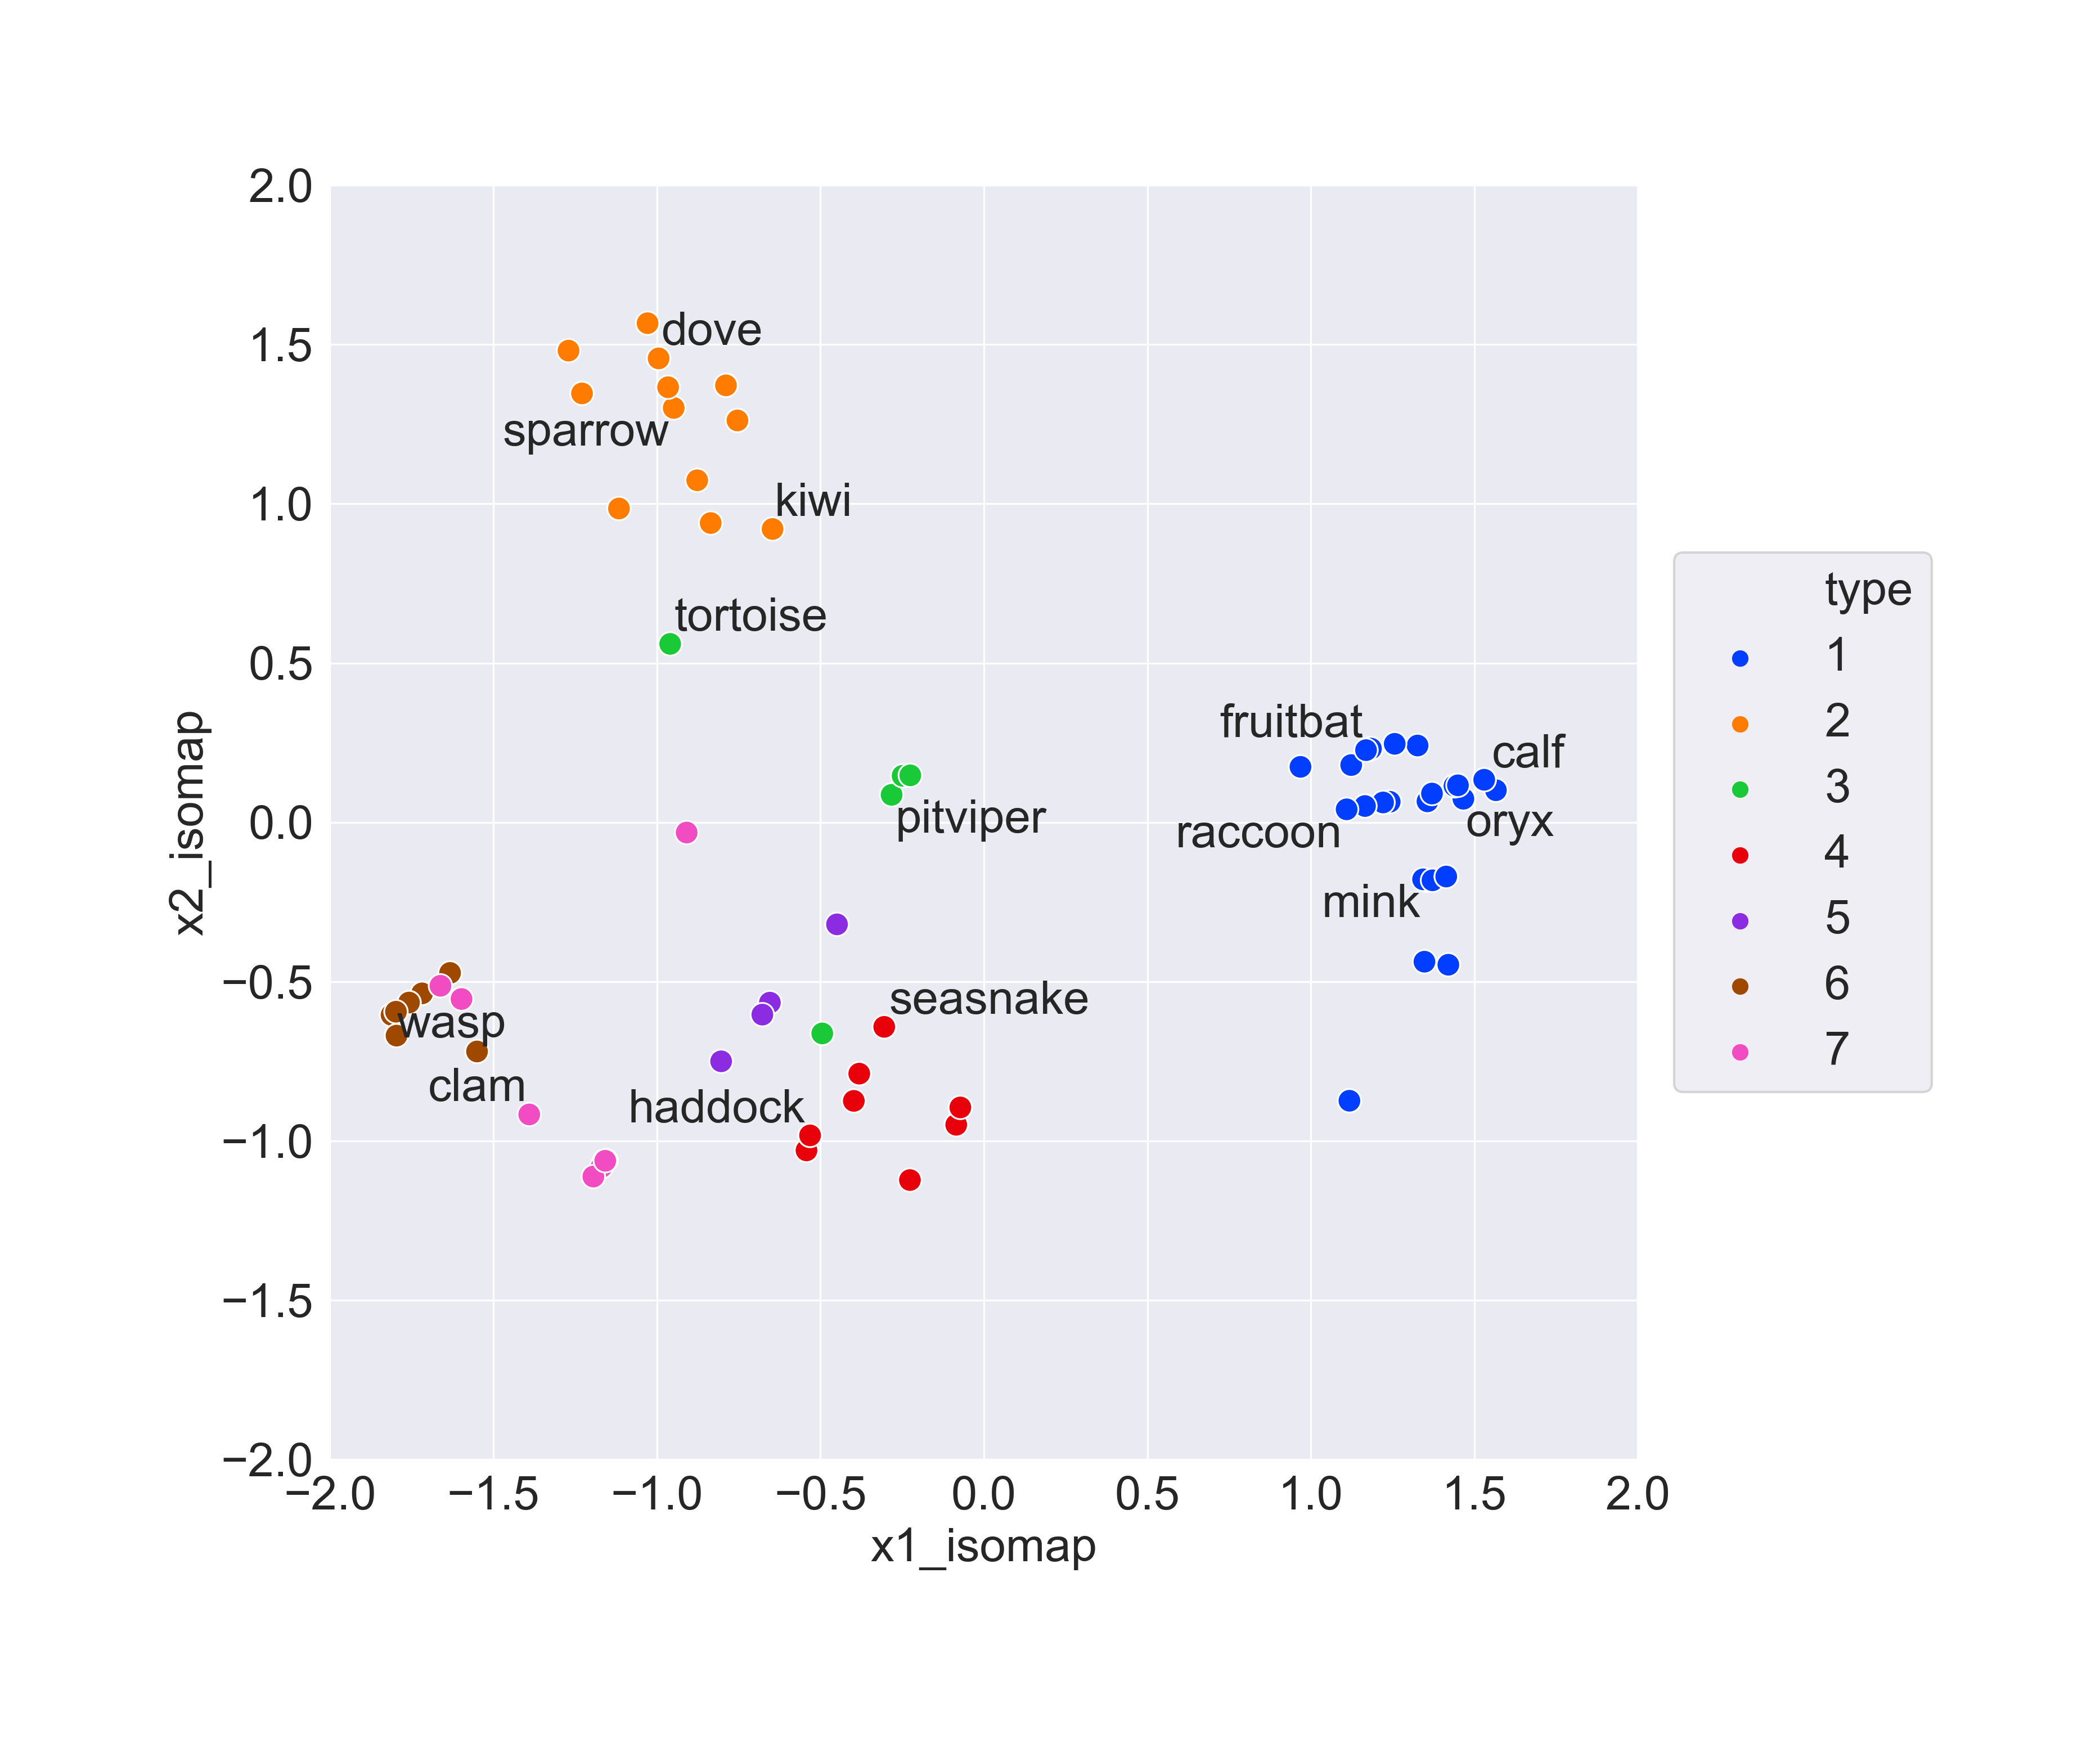
\includegraphics[width = 0.8\linewidth]{../Visualization_Isomap_n_10.png}
  \caption{Isomap, number of neighbours set to $10$}
  \label{fig:isomap 10 final}
\end{figure}

In order to make the final choice of a method I will look at how well the method captures the know relations, I.E. the relations within the designated types. This is based on the assumption that if a method correctly captures the known similarities and clusters them together it gives reason to believe that it should extrapolate well and also capture the similarities between other types of animals. Based on the plots in figures (\ref{fig:PCA final}, \ref{fig:MDS final}, \ref{fig:isomap 10 final}) Isomap perform best in clustering within types and should thus by the above assumption also be best at capturing the similarities between different types of animals. Therefore is Isomap the preferable method.
